%!TEX root = ../../super_main.tex

\section{Vision Representation}
\label{sec:vision_representation}

\todo[inline]{Det er første gang vi nævner at vores system hedder uMiner udover titel, er det fint nok?}

With the two orientation question, and hereby the four quadrants, decided upon, we have tried to to make two vision representations, namely the metaphor- and the proposition representation.

\subsection{Metaphor Representation}
\label{sub:metaphor_representation}

In Essence, metaphors are used to provide ideas by looking at some principles used in solutions for problems that are similar to your own problem. These principles can help one to find inspiration to a solution for your our problem. We have tried to define some metaphors for our problem, and the metaphors can be seen in \figref{fig:metaphor}.

\begin{figure}[!htbp]
	\centering
	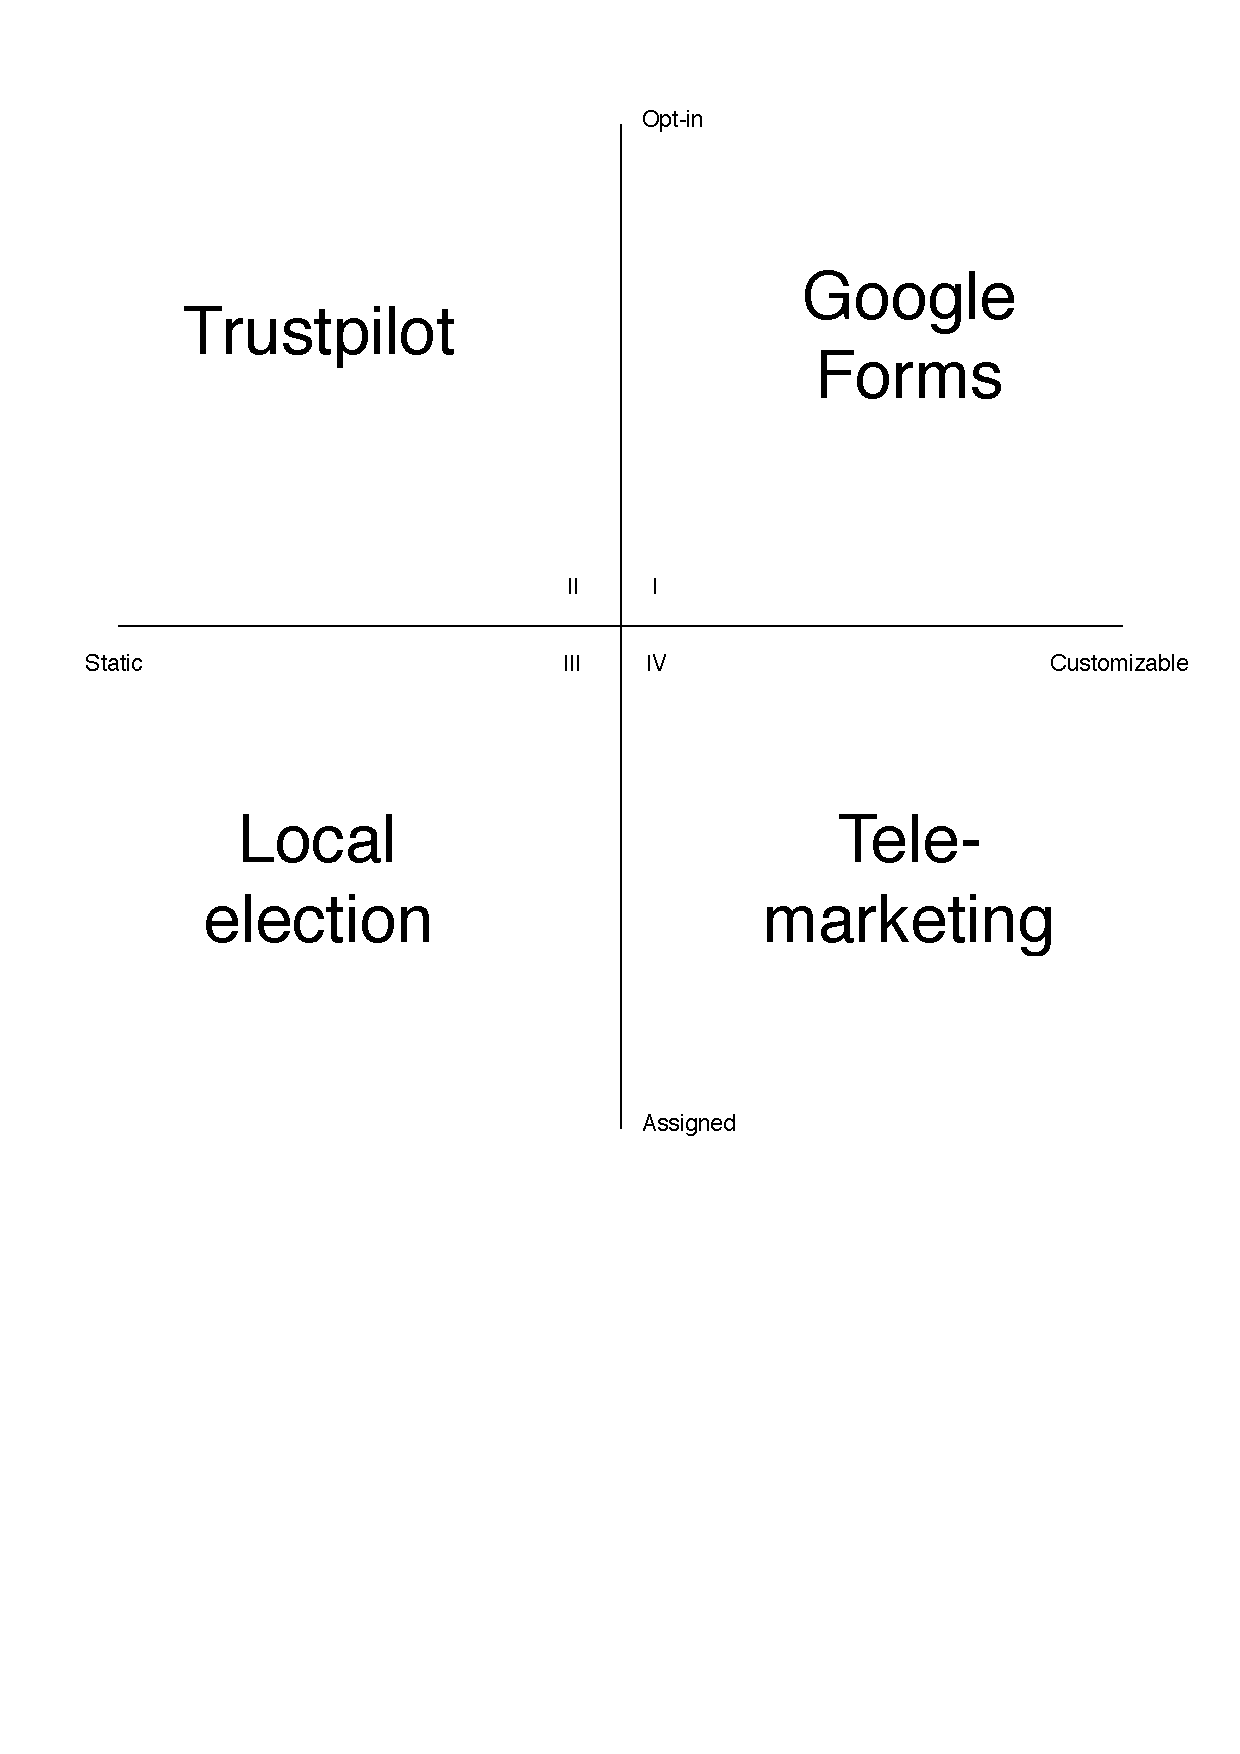
\includegraphics[width=0.8\textwidth]{graphic/problem_analysis/vision/metaphor.pdf}
	\caption{Four metaphors based upon the four quadrants.}
	\label{fig:metaphor}
\end{figure}
\FloatBarrier

The first quadrant, \emph{Google Forms}, is a survey software, where one can create a survey and distribute it. People can then choose to either answer and not to answer the questionnaire. This kind of solution can be used in our problem where participants can join a customer created campaign. The second quadrant, \emph{Trustpilot}, is a review website, where users can create reviews and rate registered online businesses. This kind solutions can be reflected to our problem, where participants can opt-in on predefined campaigns. The third quadrant, \emph{Local election}, is where the inhabitants, for a specific municipal, are selected to vote for a local election. Inhabitants who do not live in that municipal, are not allowed to vote for that local election. The voters can only vote for the candidates for the election. This kind of solution can be reflected by having a profile for each of the participants, where they are assigned the campaigns that matches their profile. The fourth quadrant, \emph{Telemarketing}, is where salespersons have profiles on potential customers. The salespersons then chooses which profiles fits best for different product they wish to sell. This kind of solution can be used in our problem, where participants gets a profile, and the customers needs to specify which kind of profiles that needs to match their own campaigns.

\subsection{Proposition Representation}
\label{sub:proposition_representation}

In Essence, a proposition is a statement or assertion that represents a design idea in a literal expression \parencite{essence_book}. Propositions can help to clarify and define scope and focus of the project. We have tried to define our design idea as propositions, where the propositions can be seen in \figref{fig:proposition}.

\begin{figure}[!htbp]
	\centering
	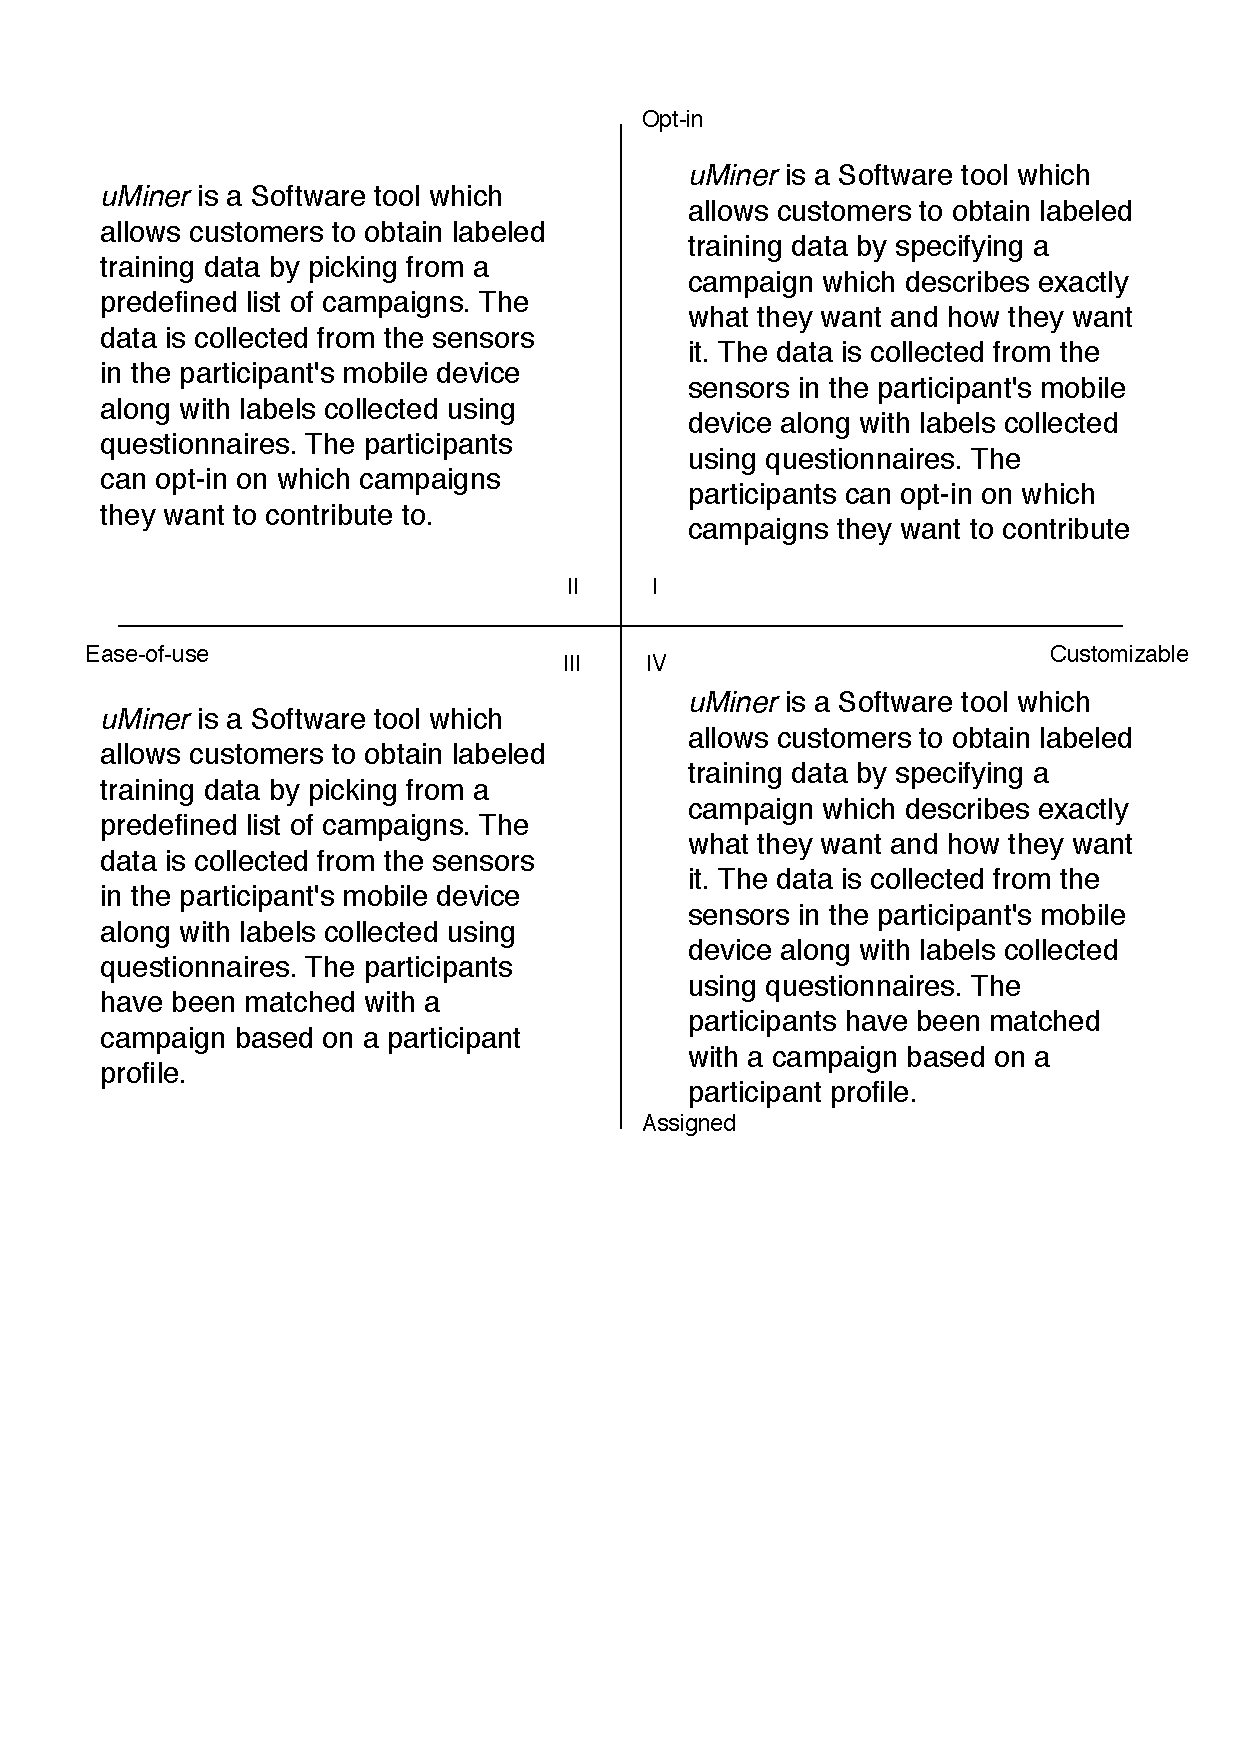
\includegraphics[width=0.8\textwidth]{graphic/problem_analysis/vision/propositions.pdf}
	\caption{Four propositions based upon the four quadrants.}
	\label{fig:proposition}
\end{figure}
\FloatBarrier

The four quadrants agrees on \emph{uMiner} to be a software tool that allows customers to acquire labeled training data. The data is collected using the participant's mobile device, and labels the data using questionnaires. The quadrants vary horizontally between either having a predefined list of campaigns the customers can pick from, or that the customers can specify their own campaigns. The quadrants vary vertically between either by having the participants to be able to opt-in on the campaigns they want to contribute to, or by having a profile for each participant and let their profiles to match with a campaign.
